\spacing{1.3}


\section{Chemical compounds}
\begin{minipage}{0.45\textwidth}
    The electrons in the outermost shell (valence electrons) are responsible for the chemical properties of an element, as shown in Figure \eqref{fig:atomo_valencia}.
    Elements that have the same electron configuration in their valence shell belong to the same group in the periodic table, which gives them similar chemical properties.

    Elements in the periodic table combine with other elements to achieve greater stability, forming chemical compounds.

\end{minipage}
\hfill
% --- Valence shell diagram (wrapfigure on the right, at section start) ---
\begin{minipage}{0.45\textwidth}
    \begin{figure}[H]
        \vspace{-12pt}
        \centering
        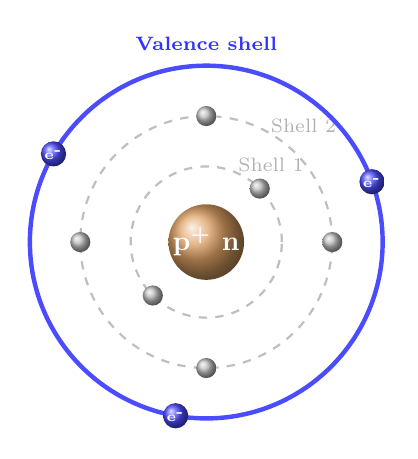
\begin{tikzpicture}[scale=0.40]
            % Nucleus with ochre gradient (only p+ and n)
            \shade[ball color=orange!80!black!60] (0,0) circle (1.2cm);
            \node[font=\normalsize\bfseries, white] at (0,0) {p\textsuperscript{+} n};
            % Shell 1 (radius 2.4)
            \draw[gray!50, thick, dashed] (0,0) circle (2.4cm);
            % Label Shell 1: between shell 1 (2.4) and shell 2 (4.0), at radius ~3.2
            \node[gray!60, font=\scriptsize] at (50:3.2) {Shell 1};
            % Shell 2 (radius 4.0, more separated)
            \draw[gray!50, thick, dashed] (0,0) circle (4.0cm);
            % Label Shell 2: between shell 2 (4.0) and valence (5.6), at radius ~4.8
            \node[gray!60, font=\scriptsize] at (50:4.8) {Shell 2};
            % Valence shell (radius 5.6, highlighted)
            \draw[blue!70, ultra thick] (0,0) circle (5.6cm);
            \node[blue!80, font=\scriptsize\bfseries] at (0, 6.3) {Valence shell};
            % Valence electrons (blue)
            \foreach \angle in {20, 150, 260} {
                \shade[ball color=blue!70] (\angle:5.6) circle (0.4cm);
                \node[white, font=\tiny\bfseries] at (\angle:5.6) {e\textsuperscript{-}};
            }
            % Inner electrons shell 1 (gray)
            \foreach \angle in {45, 225} {
                \shade[ball color=gray!50] (\angle:2.4) circle (0.32cm);
            }
            % Inner electrons shell 2 (gray)
            \foreach \angle in {0, 90, 180, 270} {
                \shade[ball color=gray!50] (\angle:4.0) circle (0.32cm);
            }
        \end{tikzpicture}
        \caption{Simplified representation of an atom.}
        \label{fig:atomo_valencia}
    \end{figure}
\end{minipage}
%
%    \begin{exercise} Answer the following questions:
%    \begin{enumerate}[label=\letraminuscula]
%        \item What are valence electrons?
%        \item Why do elements in the same group have similar chemical properties?
%        \item Sodium (\ch{Na}) and potassium (\ch{K}) are in the same group of the periodic table. Will they have similar chemical properties? Justify your answer.
%    \end{enumerate}
%    \begin{solu}
%        Answer the following questions:
%        \begin{enumerate}[label=\letraminuscula]
%        \item What are valence electrons?
%        \item Why do elements in the same group have similar chemical properties?
%        \item Sodium (\ch{Na}) and potassium (\ch{K}) are in the same group of the periodic table. Will they have similar chemical properties? Justify your answer.
%        \end{enumerate}
%        \negsubro{SOLUTION:}
%        \begin{enumerate}[label=\letraminuscula]
%            \item Valence electrons are the electrons found in the outermost shell of an atom. They are responsible for the chemical properties of the element.
%            \item Because they have the same electron configuration in their valence shell, that is, the same number of electrons in the outermost shell.
%            \item Yes, sodium and potassium will have similar chemical properties because they belong to the same group (group 1, alkali metals) and therefore have the same number of valence electrons (1 electron).
%        \end{enumerate}
%    \end{solu}
%\end{exercise}
\begin{definition}[Chemical compound]
    Is a substance formed by two or more different elements that are chemically bonded in fixed proportions.
\end{definition}
It is also important to know the definition of molecule.
\begin{definition}[Molecule]
    is the smallest unit of a chemical substance that retains its properties.
\end{definition}
The different types of structures we can find are:
\begin{enumerate}[label=\numberballmDarkTeal]
        \item \negsubro{Isolated atoms}. \\
        Isolated atoms are found in \textbf{noble gases} due to their high stability.
        Noble gases do not tend to combine with other elements because their valence shell is already complete.

        Isolated atoms have the following \textbf{physical and chemical properties}:
        \begin{itemize}
            \item They are gaseous substances at room temperature.
            \item They do not conduct electricity.
            \item They do not react with other substances.
        \end{itemize}

        \item \negsubro{Homonuclear diatomic molecules}. \\
        These are molecules formed by two atoms of the same element.
        The homonuclear diatomic molecules found in nature are:
        \ch{H2}, \ch{O2}, \ch{N2}, \ch{F2}, \ch{Cl2}, \ch{Br2}, and \ch{I2}.

        \item \negsubro{Heteronuclear molecules}. \\
        These are molecules that contain two or more different elements.

        Examples: \ch{HCl}, \ch{H2S}, \ch{H2O}.

        \item \negsubro{Crystals}. \\
        These are solids whose particles are arranged following a pattern that repeats in all three dimensions of space.
        \begin{itemize}
            \item \textbf{Non-metallic crystals}: such as graphite and diamond, both formed by carbon but with different structures.
            \item \textbf{Metallic crystals}: such as iron, copper, etc.
        \end{itemize}

        % --- Comparative diagram: diamond vs graphite ---
        Figure \eqref{fig:diamante_grafito} shows how carbon can form two very different crystalline structures.

        \begin{figure}[ht]
            \centering
            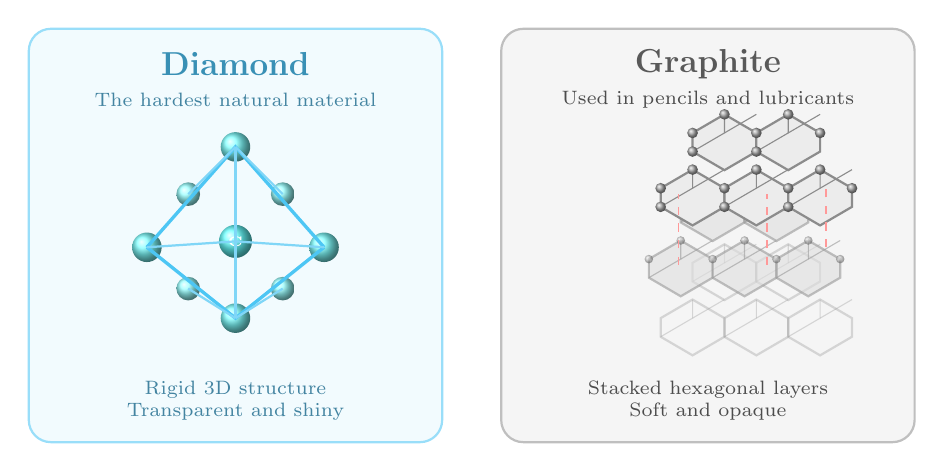
\begin{tikzpicture}[scale=0.75]
                % ===== DIAMOND =====
                % Decorative frame
                \fill[cyan!5, rounded corners=8pt] (-7.5,-1.8) rectangle (-0.5,5.2);
                \draw[cyan!40, thick, rounded corners=8pt] (-7.5,-1.8) rectangle (-0.5,5.2);
                \node[font=\large\bfseries, cyan!70!black] at (-4, 4.6) {Diamond};
                % Hardness icon
                \node[font=\scriptsize, cyan!60!black] at (-4, 4.0) {The hardest natural material};
                % 3D tetrahedral structure with perspective
                % Carbon atoms (shiny spheres)
                \shade[ball color=cyan!50] (-5.5,1.5) circle (0.25);
                \shade[ball color=cyan!50] (-2.5,1.5) circle (0.25);
                \shade[ball color=cyan!50] (-4,3.2) circle (0.25);
                \shade[ball color=cyan!50] (-4,0.3) circle (0.25);
                \shade[ball color=cyan!40] (-4.8,2.4) circle (0.2);

                \shade[ball color=cyan!40] (-3.2,2.4) circle (0.2);
                \shade[ball color=cyan!40] (-4.8,0.8) circle (0.2);
                \shade[ball color=cyan!40] (-3.2,0.8) circle (0.2);
                \shade[ball color=cyan!60] (-4,1.6) circle (0.28);
                \node[white, font=\tiny\bfseries] at (-4,1.6) {C};
                % Strong bonds (thick lines)
                \draw[cyan!70, very thick] (-5.5,1.5)--(-4,3.2)--(-2.5,1.5);
                \draw[cyan!70, very thick] (-5.5,1.5)--(-4,0.3)--(-2.5,1.5);
                \draw[cyan!70, very thick] (-4,3.2)--(-4,0.3);
                \draw[cyan!50, thick] (-4,1.6)--(-5.5,1.5);
                \draw[cyan!50, thick] (-4,1.6)--(-2.5,1.5);
                \draw[cyan!50, thick] (-4,1.6)--(-4,3.2);
                \draw[cyan!50, thick] (-4,1.6)--(-4,0.3);
                \draw[cyan!50, thick] (-4.8,2.4)--(-4,3.2);
                \draw[cyan!50, thick] (-3.2,2.4)--(-4,3.2);
                \draw[cyan!50, thick] (-4.8,0.8)--(-4,0.3);
                \draw[cyan!50, thick] (-3.2,0.8)--(-4,0.3);
                % Properties
                \node[font=\scriptsize, text width=3cm, align=center, cyan!60!black] at (-4,-1.1) {Rigid 3D structure \\ Transparent and shiny};

                % ===== GRAPHITE =====
                \fill[gray!8, rounded corners=8pt] (0.5,-1.8) rectangle (7.5,5.2);
                \draw[gray!50, thick, rounded corners=8pt] (0.5,-1.8) rectangle (7.5,5.2);
                \node[font=\large\bfseries, gray!70!black] at (4, 4.6) {Graphite};
                \node[font=\scriptsize, gray!60!black] at (4, 4.0) {Used in pencils and lubricants};
                % Lower layer (lighter, depth effect)
                \begin{scope}[shift={(3.2,0.3)}, scale=0.9, opacity=0.35]
                    \foreach \hx/\hy in {0/0, 1.2/0, 2.4/0, 0.6/1.04, 1.8/1.04} {
                        \draw[gray!80, thick]
                        (\hx,\hy) -- ++(0.6,0.35) -- ++(0.6,-0.35)
                        -- ++(0,-0.35) -- ++(-0.6,-0.35) -- ++(-0.6,0.35) -- cycle;
                        \draw[gray!80] (\hx+0.6,\hy+0.35) -- ++(0,-0.35) -- ++(-0.6,-0.35);
                        \draw[gray!80] (\hx+0.6,\hy) -- ++(0.6,0.35);
                    }
                \end{scope}
                % Middle layer
                \begin{scope}[shift={(3.0,1.3)}, scale=0.9, opacity=0.6]
                    \foreach \hx/\hy in {0/0, 1.2/0, 2.4/0, 0.6/1.04, 1.8/1.04} {
                        \fill[gray!25]
                        (\hx,\hy) -- ++(0.6,0.35) -- ++(0.6,-0.35)
                        -- ++(0,-0.35) -- ++(-0.6,-0.35) -- ++(-0.6,0.35) -- cycle;
                        \draw[gray!80, thick]
                        (\hx,\hy) -- ++(0.6,0.35) -- ++(0.6,-0.35)
                        -- ++(0,-0.35) -- ++(-0.6,-0.35) -- ++(-0.6,0.35) -- cycle;
                        \draw[gray!80] (\hx+0.6,\hy+0.35) -- ++(0,-0.35) -- ++(-0.6,-0.35);
                        \draw[gray!80] (\hx+0.6,\hy) -- ++(0.6,0.35);
                    }
                    % Atoms at vertices of middle layer
                    \foreach \ax/\ay in {0/0, 0.6/0.35, 1.2/0, 1.8/0.35, 2.4/0, 3.0/0.35, 3.6/0,
                    0.6/1.04, 1.2/1.39, 1.8/1.04, 2.4/1.39, 3.0/1.04} {
                        \shade[ball color=gray!55] (\ax,\ay) circle (0.08);
                    }
                \end{scope}
                % Top layer (darker, foreground)
                \begin{scope}[shift={(3.2,2.5)}, scale=0.9]
                    \foreach \hx/\hy in {0/0, 1.2/0, 2.4/0, 0.6/1.04, 1.8/1.04} {
                        \fill[gray!15]
                        (\hx,\hy) -- ++(0.6,0.35) -- ++(0.6,-0.35)
                        -- ++(0,-0.35) -- ++(-0.6,-0.35) -- ++(-0.6,0.35) -- cycle;
                        \draw[gray!90, thick]
                        (\hx,\hy) -- ++(0.6,0.35) -- ++(0.6,-0.35)
                        -- ++(0,-0.35) -- ++(-0.6,-0.35) -- ++(-0.6,0.35) -- cycle;
                        \draw[gray!90] (\hx+0.6,\hy+0.35) -- ++(0,-0.35) -- ++(-0.6,-0.35);
                        \draw[gray!90] (\hx+0.6,\hy) -- ++(0.6,0.35);
                    }
                    % Atoms at vertices of top layer
                    \foreach \ax/\ay in {0/0, 0.6/0.35, 1.2/0, 1.8/0.35, 2.4/0, 3.0/0.35, 3.6/0,
                    0/-0.35, 1.2/-0.35, 2.4/-0.35,
                    0.6/1.04, 1.2/1.39, 1.8/1.04, 2.4/1.39, 3.0/1.04,
                    0.6/0.69, 1.8/0.69} {
                        \shade[ball color=gray!70] (\ax,\ay) circle (0.1);
                    }
                \end{scope}
                % Separation lines between layers (weak forces)
                \draw[red!40, dashed, thin] (3.5,1.2) -- (3.5,2.4);
                \draw[red!40, dashed, thin] (5.0,1.2) -- (5.0,2.4);
                \draw[red!40, dashed, thin] (6.0,1.5) -- (6.0,2.6);
                % Properties
                \node[font=\scriptsize, text width=4cm, align=center, gray!60!black] at (4,-1.1) {Stacked hexagonal layers \\ Soft and opaque};
            \end{tikzpicture}
            \caption{Diamond and graphite are both made of carbon, but their different structures give them very different properties.}
            \label{fig:diamante_grafito}
        \end{figure}
\end{enumerate}


\section{Chemical bonding}

Atoms of different elements join together to form molecules. This union is called a \azul{\texttt{chemical bond}}. Chemical bonding occurs because the molecule formed is more stable than the isolated atoms.

In nature we can mainly find 3 types of bonds:

\begin{enumerate}[label=\numberballmDarkTeal]
\item \negsubro{Ionic bond}: occurs by electron transfer. One element loses electrons and another gains them, forming a cation (positive ion) and an anion (negative ion). Both ions are held together by the electric force of attraction.

For example, \ch{NaCl} forms because \ch{Na} loses one \el{} and becomes \ch{Na+}, while \ch{Cl} gains that \el{} and becomes \ch{Cl-}, resulting in \ch{Na+ Cl-} (Figure \eqref{fig:enlace_ionico}).

% --- Ionic bond diagram ---
\begin{figure}[ht]
    \centering
    \begin{tikzpicture}[scale=0.85]
% Title
        \node[font=\bfseries\large, orange!70!black] at (1.5,3.9) {Formation of the ionic bond: \ch{NaCl}};

% === BEFORE ===
        \node[font=\small\bfseries, gray] at (-5.5,2.3) {BEFORE};

% Na with electron shells
        \shade[ball color=blue!40] (-4.5,0) circle (0.6);
        \node[white, font=\bfseries] at (-4.5,0) {Na};
% Na valence shell (1 electron)
        \draw[blue!50, thick] (-4.5,0) circle (1.3);
        \shade[ball color=red!70] (-4.5,1.3) circle (0.15);
        \node[font=\tiny, blue!70] at (-4.5,-1.7) {11 e\textsuperscript{-} (2, 8, \textbf{1})};

% Cl with electron shells
        \shade[ball color=green!60!black!40] (-1.5,0) circle (0.7);
        \node[white, font=\bfseries] at (-1.5,0) {Cl};
% Cl valence shell (7 electrons)
        \draw[green!60!black, thick] (-1.5,0) circle (1.4);
        \foreach \a in {0,51.4,102.8,154.3,205.7,257.1,308.6} {
            \shade[ball color=red!70] ({-1.5+1.4*cos(\a)},{1.4*sin(\a)}) circle (0.15);
        }
        \node[font=\tiny, green!50!black] at (-1.5,-1.7) {17 e\textsuperscript{-} (2, 8, \textbf{7})};

% Transfer arrow (curved, with correct tip)
        \draw[-{Stealth[length=8pt, width=5pt]}, ultra thick, red!70, decorate, decoration={snake, amplitude=1.5pt, segment length=8pt, post length=8pt}]
        (-4.5,1.6) .. controls (-3,2.8) and (-2,2.8) .. (-1.5,1.7);
        \node[font=\small\bfseries, red!70] at (-3,3.0) {1 e\textsuperscript{-}};

% === Central arrow ===
        \draw[->, ultra thick, orange!70, >=stealth] (0.8,0) -- (2.2,0);
        \node[font=\tiny\bfseries, orange!70] at (1.5,0.4) {Forms};

% === AFTER ===
        \node[font=\small\bfseries, gray] at (5.5,2.3) {AFTER};

% Na+ (smaller, lost electron)
        \shade[ball color=blue!60] (4,0) circle (0.5);
        \node[white, font=\bfseries] at (4,0) {Na\textsuperscript{+}};
% Decorative + sign
        \node[blue!70, font=\Large\bfseries] at (4,1.0) {$+$};

% Cl- (larger, gained electron)
        \shade[ball color=green!60!black!40] (7,0) circle (0.8);
        \node[white, font=\bfseries] at (7,0) {Cl\textsuperscript{-}};
% Decorative - sign
        \node[green!50!black, font=\Large\bfseries] at (7,1.2) {$-$};

% Attraction force (rays)
        \foreach \dy in {-0.3,0,0.3} {
            \draw[orange!80, thick, <->, >=stealth] (4.6,\dy) -- (6.1,\dy);
        }
        \node[font=\tiny\bfseries, orange!80] at (5.35,-0.8) {Electric attraction};

% Final configuration
        \node[font=\tiny, blue!70] at (4,-1.7) {10 e\textsuperscript{-} (2, 8)};
        \node[font=\tiny, green!50!black] at (7,-1.7) {18 e\textsuperscript{-} (2, 8, 8)};

% Stability note
        \node[font=\tiny, gray, text width=3cm, align=center] at (5.5,-2.8) {Both now have \\ 8 e\textsuperscript{-} in their outermost shell};
    \end{tikzpicture}
    \caption{Formation of the ionic bond in \ch{NaCl}. Sodium transfers one electron to chlorine, forming ions that attract each other.}
    \label{fig:enlace_ionico}
\end{figure}

\item \negsubro{Covalent bond}: this is the bond that forms when two atoms share electrons. The bond formed is represented with a line (\ch{-}), although it is sometimes omitted for simplicity.

For example, \ch{H} and \ch{Cl} share electrons to form a covalent bond: \ch{H-Cl} (Figure \eqref{fig:enlace_covalente}).

% --- Covalent bond diagram ---
\begin{figure}[ht]
    \centering
    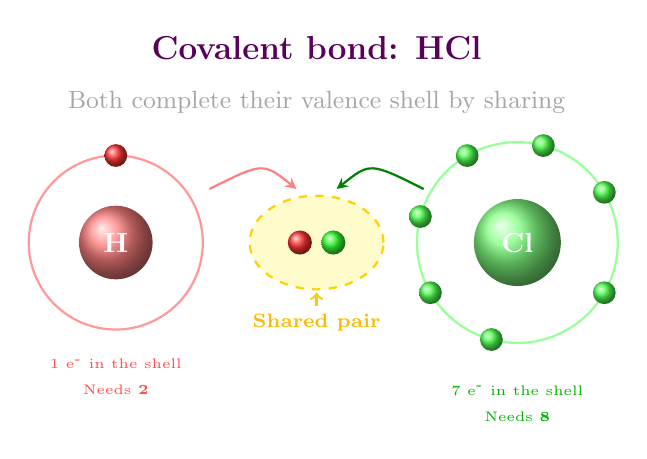
\begin{tikzpicture}[scale=0.85]
% Background
%\fill[violet!3, rounded corners=10pt] (-6,-3.5) rectangle (6,3.5);
% Title
        \node[font=\bfseries\large, violet!70!black] at (0,2.9) {Covalent bond: \ch{HCl}};

% === H (left) ===
% H electron shell
        \draw[red!40, thick] (-3,0) circle (1.3);
        \shade[ball color=red!50] (-3,0) circle (0.55);
        \node[white, font=\bfseries] at (-3,0) {H};
% H's own electron
        \shade[ball color=red!80] (-3,1.3) circle (0.17);
        \node[font=\tiny, red!70] at (-3,-1.8) {1 e\textsuperscript{-} in the shell};
        \node[font=\tiny, red!70] at (-3,-2.2) {Needs \textbf{2}};

% === Cl (right) ===
        \draw[green!40, thick] (3,0) circle (1.5);
        \shade[ball color=green!50] (3,0) circle (0.65);
        \node[white, font=\bfseries] at (3,0) {Cl};
% Cl's 7 valence electrons
        \foreach \a/\c in {30/green!70, 75/green!70, 120/green!70, 165/green!70, 210/green!70, 255/green!70, 330/green!70} {
            \shade[ball color=\c] ({3+1.5*cos(\a)},{1.5*sin(\a)}) circle (0.17);
        }
        \node[font=\tiny, green!70!black] at (3,-2.2) {7 e\textsuperscript{-} in the shell};
        \node[font=\tiny, green!70!black] at (3,-2.6) {Needs \textbf{8}};

% === Sharing zone (center) ===
        \fill[yellow!40, opacity=0.5] (0,0) ellipse (1.0 and 0.7);
        \draw[yellow!70!orange, thick, dashed] (0,0) ellipse (1.0 and 0.7);
% Shared electron pair
        \shade[ball color=red!80] (-0.25,0) circle (0.18);
        \shade[ball color=green!80] (0.25,0) circle (0.18);
% Label
        \node[font=\scriptsize\bfseries, yellow!50!orange, fill=white, inner sep=2pt, rounded corners] at (0,-1.2) {Shared pair};
        \draw[->, yellow!60!orange, thick] (0,-0.95) -- (0,-0.75);

% Approach arrows
        \draw[->, thick, red!50, >=stealth] (-1.6,0.8) .. controls (-0.8,1.2) .. (-0.3,0.8);
        \draw[->, thick, green!50!black, >=stealth] (1.6,0.8) .. controls (0.8,1.2) .. (0.3,0.8);

% Result below
        \node[font=\small, gray!70, fill=white, inner sep=3pt, rounded corners=3pt] at (0,2.1)
            {Both complete their valence shell by sharing};
    \end{tikzpicture}
    \caption{Covalent bond in \ch{HCl}. Both atoms share an electron pair to complete their valence shell.}
    \label{fig:enlace_covalente}
\end{figure}

\item \negsubro{Metallic bond}: this is the bond that forms between atoms of metallic elements. The atoms of a metal share their valence electrons, which move freely among all the atoms forming an ``electron cloud''. This explains why metals conduct electricity.

% --- Metallic bond diagram ---
Figure \eqref{fig:enlace_metalico} illustrates this type of bond.

\begin{figure}[ht]
    \centering
    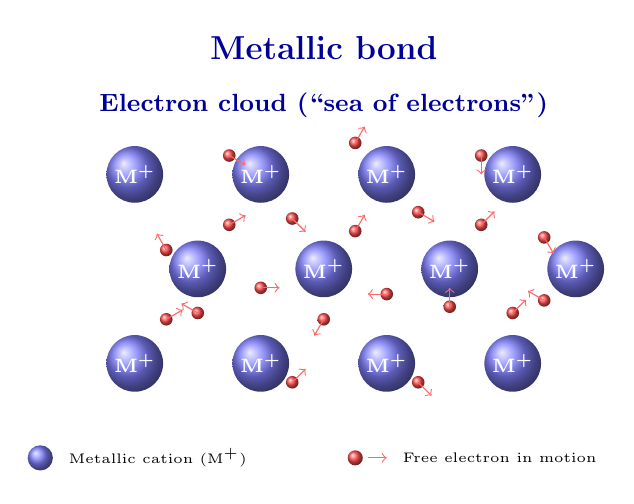
\begin{tikzpicture}[scale=0.8]
% General background
%\fill[blue!3, rounded corners=10pt] (-3.5,-3.5) rectangle (7.5,4.5);
% Title
        \node[font=\bfseries\large, blue!60!black] at (2,3.5) {Metallic bond};

% Electron cloud (vibrant yellow background)
%\fill[yellow!25, rounded corners=12pt] (-2.5,-2.5) rectangle (6.5,3.0);
%\fill[yellow!15, rounded corners=12pt] (-2.8,-2.8) rectangle (6.8,3.2);
%\draw[yellow!60, thick, dashed, rounded corners=12pt] (-2.8,-2.8) rectangle (6.8,3.2);
        \node[font=\small\bfseries, blue!60!black, inner sep=3pt, rounded corners=3pt] at (2,2.6) {Electron cloud (``sea of electrons'')};

% Lattice of metallic cations (ordered arrangement)
        \foreach \x/\y in {-1/-1.5, 1/-1.5, 3/-1.5, 5/-1.5, 0/0, 2/0, 4/0, 6/0, -1/1.5, 1/1.5, 3/1.5, 5/1.5} {
            \shade[ball color=blue!50] (\x,\y) circle (0.45);
            \node[white, font=\scriptsize\bfseries] at (\x,\y) {M\textsuperscript{+}};
        }

% Free electrons moving (with arrows to indicate movement)
        \foreach \x/\y/\ang in {
            0.5/0.7/30, 1.5/0.8/-45, 2.5/0.6/60, 3.5/0.9/-30,
            4.5/0.7/45, -0.5/0.3/120, 5.5/0.5/-60,
            0/-0.7/150, 2/-0.8/-120, 4/-0.6/90,
            1/-0.3/0, 3/-0.4/180, 5/-0.7/45,
            0.5/1.8/-30, 2.5/2.0/60, 4.5/1.8/-90,
            -0.5/-0.8/30, 5.5/-0.5/150, 1.5/-1.8/45, 3.5/-1.8/-45
        } {
            \shade[ball color=red!70] (\x,\y) circle (0.1);
            \draw[->, red!60, thin] (\x,\y) -- ++(\ang:0.3);
        }

% Legend
        \shade[ball color=blue!50] (-2.5,-3.0) circle (0.2);
        \node[font=\tiny, right] at (-2.2,-3.0) {Metallic cation (M\textsuperscript{+})};
        \shade[ball color=red!70] (2.5,-3.0) circle (0.12);
        \draw[->, red!60, thin] (2.7,-3.0) -- ++(0:0.3);
        \node[font=\tiny, right] at (3.1,-3.0) {Free electron in motion};
    \end{tikzpicture}
    \caption{In the metallic bond, metal cations are surrounded by a cloud of free-moving electrons, which explains electrical conductivity.}
    \label{fig:enlace_metalico}
\end{figure}

\end{enumerate}


\section{Atomic mass and molecular mass}

\subsection{Atomic mass}
Atoms are very small particles, so if we measured their mass in kilograms, we would get extremely small values. That is why a special unit was created that allows us to work with these masses more easily.

This unit is called \azul{\texttt{atomic mass unit (amu)}} and is represented by \unit{\uma}.

\begin{definition}[Atomic mass unit]
    It is one-twelfth (\( \frac{1}{12} \)) of the mass of a \isotope{C} atom. We can say that \( \qty{1}{\uma} \approx \qty{1.67e-27}{\kilogram} \).
\end{definition}

In many cases, the atomic mass unit is omitted and only the number is given.

In the periodic table we can find the atomic masses of each element in amu.

If we wanted to know the mass of an atom in kilograms, we would have to convert amu to kilograms using the equivalence given above.

\subsection{Molecular mass}

If what we have is a molecule, we must calculate its molecular mass, that is, the sum of the atomic masses of all the atoms that make up that molecule. Molecular mass is also expressed in amu.

\begin{example}{}
    Let's calculate the molecular mass of \ch{H2O} knowing that the atomic masses of the elements are \( \ch{H} = 1 \) and \( \ch{O} = 16 \).
    \[
        \ch{H2O} \left\{\rule{0pt}{0.8cm}
                     \begin{array}{lcl}
                         \ch{H} &=& 2 \times \qty{1}{\uma} = \qty{2}{\uma} \\
                         \ch{O} &=& 1 \times \qty{16}{\uma} = \qty{16}{\uma} \\
                         \cline{1-3}
                         \multicolumn{3}{r}{\textbf{Total} = \qty{18}{\uma}}
                     \end{array}
        \right.
    \]
\end{example}

\begin{example}{}
    Let's calculate the molecular mass of \ch{H2SO4} knowing that the atomic masses of the elements are \( \ch{H} = 1 \), \( \ch{O} = 16 \), and \( \ch{S} = 32 \).
    \[
        \ch{H2SO4} \left\{\rule{0pt}{0.8cm}
                       \begin{array}{lcl}
                           \ch{H} &=& 2 \times \qty{1}{\uma} = \qty{2}{\uma} \\
                           \ch{S} &=& 1 \times \qty{32}{\uma} = \qty{32}{\uma} \\
                           \ch{O} &=& 4 \times \qty{16}{\uma} = \qty{64}{\uma} \\
                           \cline{1-3}
                           \multicolumn{3}{r}{\textbf{Total} = \qty{98}{\uma}}
                       \end{array}
        \right.
    \]
\end{example}



\begin{exercise}
    Indicate which is the correct way to calculate the molecular mass of calcium sulfate, \ch{CaSO4}:
    \begin{enumerate}[label=\letraminuscula]
\item Atomic mass of calcium + atomic mass of sulfur + atomic mass of oxygen.
\item Atomic mass of calcium + atomic mass of sulfur + four times the atomic mass of oxygen.
    \end{enumerate}
    \begin{solu}
        Indicate which is the correct way to calculate the molecular mass of calcium sulfate, \ch{CaSO4}:
        \begin{enumerate}[label=\letraminuscula]
\item Atomic mass of calcium + atomic mass of sulfur + atomic mass of oxygen.
\item Atomic mass of calcium + atomic mass of sulfur + four times the atomic mass of oxygen.
        \end{enumerate}
        Indicate which is the correct way to calculate the molecular mass of calcium sulfate, \ch{CaSO4}:

        The correct answer is \textbf{b)}: atomic mass of calcium + atomic mass of sulfur + four times the atomic mass of oxygen.

        In the formula \ch{CaSO4}, the subscript 4 indicates that there are 4 oxygen atoms, so we must multiply the atomic mass of oxygen by 4.
    \end{solu}
\end{exercise}

\begin{exercise}
    Air, mainly composed of nitrogen (\ch{N2}) and oxygen (\ch{O2}), contains variable amounts of carbon dioxide (\ch{CO2}). Look up the atomic masses in the periodic table and calculate the molecular mass of these three gases.
    \begin{solu}
        Air, mainly composed of nitrogen (\ch{N2}) and oxygen (\ch{O2}), contains variable amounts of carbon dioxide (\ch{CO2}). Look up the atomic masses in the periodic table and calculate the molecular mass of these three gases.
        Calculate the molecular mass of \ch{N2}, \ch{O2}, and \ch{CO2}.

        Atomic masses: \( \ch{N} = 14 \); \( \ch{O} = 16 \); \( \ch{C} = 12 \).

        \begin{itemize}
            \item \ch{N2}: \( 2 \times 14 = \qty{28}{\uma} \)
            \item \ch{O2}: \( 2 \times 16 = \qty{32}{\uma} \)
            \item \ch{CO2}: \( 1 \times 12 + 2 \times 16 = 12 + 32 = \qty{44}{\uma} \)
        \end{itemize}
    \end{solu}
\end{exercise}

\begin{exercise}
    Calculate the molecular mass of zinc oxide (\ch{ZnO}), potassium nitrate (\ch{KNO3}), calcium sulfate (\ch{CaSO4}), butane (\ch{C4H10}), and calcium carbonate (\ch{CaCO3}).
    \begin{solu}
        Calculate the molecular mass of zinc oxide (\ch{ZnO}), potassium nitrate (\ch{KNO3}), calcium sulfate (\ch{CaSO4}), butane (\ch{C4H10}), and calcium carbonate (\ch{CaCO3}).

        Calculate the molecular mass of \ch{ZnO}, \ch{KNO3}, \ch{CaSO4}, \ch{C4H10}, and \ch{CaCO3}.

        Atomic masses: \( \ch{Zn} = 65 \); \( \ch{O} = 16 \); \( \ch{K} = 39 \); \( \ch{N} = 14 \); \( \ch{Ca} = 40 \); \( \ch{S} = 32 \); \( \ch{C} = 12 \); \( \ch{H} = 1 \).
        \begin{itemize}
            \item \ch{ZnO}: \( 65 + 16 = \qty{81}{\uma} \)
            \item \ch{KNO3}: \( 39 + 14 + 3 \times 16 = 39 + 14 + 48 = \qty{101}{\uma} \)
            \item \ch{CaSO4}: \( 40 + 32 + 4 \times 16 = 40 + 32 + 64 = \qty{136}{\uma} \)
            \item \ch{C4H10}: \( 4 \times 12 + 10 \times 1 = 48 + 10 = \qty{58}{\uma} \)
            \item \ch{CaCO3}: \( 40 + 12 + 3 \times 16 = 40 + 12 + 48 = \qty{100}{\uma} \)
        \end{itemize}
    \end{solu}
\end{exercise}

\begin{exercise}
    Look up the atomic masses in the periodic table of this unit and arrange the following compounds from highest to lowest oxygen percentage: \ch{BaO}, \ch{K2O}, and \ch{CO2}.
    \begin{solu}
        Look up the atomic masses in the periodic table of this unit and arrange the following compounds from highest to lowest oxygen percentage: \ch{BaO}, \ch{K2O}, and \ch{CO2}.

        Arrange \ch{BaO}, \ch{K2O}, and \ch{CO2} from highest to lowest oxygen percentage.

        Atomic masses: \( \ch{Ba} = 137 \); \( \ch{K} = 39 \); \( \ch{C} = 12 \); \( \ch{O} = 16 \).

        \begin{itemize}
            \item \ch{BaO}: molecular mass \( = 137 + 16 = \qty{153}{\uma} \). Percentage of O \( = \frac{16}{153} \times 100 = 10.5 \% \)
            \item \ch{K2O}: molecular mass \( = 2 \times 39 + 16 = \qty{94}{\uma} \). Percentage of O \( = \frac{16}{94} \times 100 = 17{,}0\% \)
            \item \ch{CO2}: molecular mass \( = 12 + 2 \times 16 = \qty{44}{\uma} \). Percentage of O \( = \frac{32}{44} \times 100 = 72{,}7\% \)
        \end{itemize}

        Order from highest to lowest oxygen percentage: \ch{CO2} > \ch{K2O} > \ch{BaO}.
    \end{solu}
\end{exercise}


\begin{exercise}
    Indicate which of these two substances has a higher percentage of potassium: potassium chloride (\ch{KCl}) or potassium nitrate (\ch{KNO3}).
    \begin{solu}
        Indicate which of these two substances has a higher percentage of potassium: potassium chloride (\ch{KCl}) or potassium nitrate (\ch{KNO3}).

        Which has a higher percentage of potassium, \ch{KCl} or \ch{KNO3}?

        Atomic masses: \( \ch{K} = 39 \); \( \ch{Cl} = 35{,}5 \); \( \ch{N} = 14 \); \( \ch{O} = 16 \).

        \begin{itemize}
            \item \ch{KCl}: molecular mass \( = 39 + \num{35.5} = \qty{74.5}{\uma} \). Percentage of K \( = \frac{39}{74.5} \times 100 = 52.3\% \)
            \item \ch{KNO3}: molecular mass \( = 39 + 14 + 3 \times 16 = \qty{101}{\uma} \). Percentage of K \( = \frac{39}{101} \times 100 = 38.6\% \)
        \end{itemize}

        \ch{KCl} has a higher percentage of potassium (52.3\,\%) than \ch{KNO3} (38.6\,\%).
    \end{solu}
\end{exercise}


\section{Amount of substance: the mole}

Since atoms are very small and matter is made up of enormous quantities of them, a unit was created to group many atoms together so we can work with amounts that are easier to handle.

For this purpose, the unit of substance called \azul{\texttt{mole}} was created and is represented by \( \bm{n} \).

\begin{definition}[Mole]
    It is the amount of substance that contains \num{6.022e23} elementary entities, which can be atoms, molecules, ions, electrons, or other particles.
\end{definition}

We can understand the mole as a ``box'' that always holds \num{6.022e23} ``things''.

This very large number is called \azul{\texttt{Avogadro's constant}} and is represented by \( \bm{N_A} \).

\begin{equation*}
    N_A = \num{6.022e23}\ \dfrac{\text{particles}}{\unit{\mol}}
\end{equation*}

% --- Visual diagram of the mole ---
Figure \eqref{fig:mol_particulas} illustrates this concept.

\begin{figure}[ht]
    \centering
    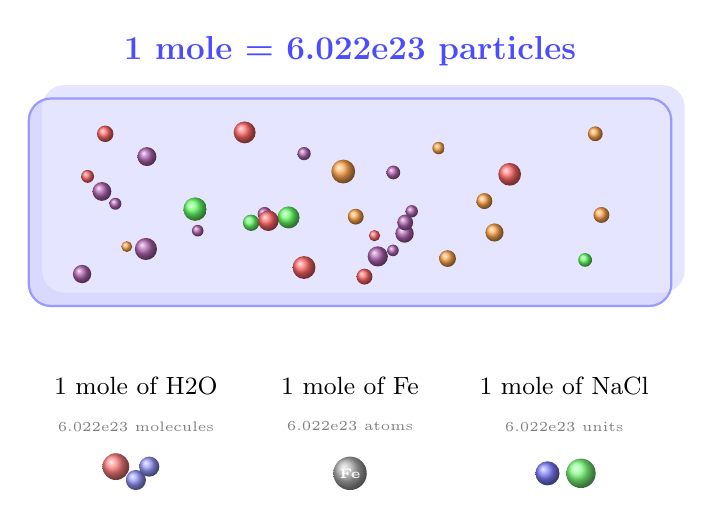
\begin{tikzpicture}[scale=0.85]
% General background
%\fill[blue!3, rounded corners=12pt] (-5.5,-3.5) rectangle (5.5,4.5);

% Large title
        \node[font=\large\bfseries, blue!70] at (0,3.5) {1 mole = \num{6.022e23} particles};

% Main box with 3D effect
        \fill[blue!15, rounded corners=8pt] (-4.8,-0.3) rectangle (4.8,2.8);
        \fill[blue!10, rounded corners=8pt] (-4.6,-0.1) rectangle (5.0,3.0);
        \draw[blue!40, thick, rounded corners=8pt] (-4.8,-0.3) rectangle (4.8,2.8);

% Particles of various colors and sizes to make it visual
        \pgfmathsetseed{42}
        \foreach \i in {1,...,35} {
            \pgfmathsetmacro{\rx}{-4.2 + rnd*8.0}
            \pgfmathsetmacro{\ry}{0.1 + rnd*2.2}
            \pgfmathsetmacro{\rr}{0.08 + rnd*0.1}
            \pgfmathsetmacro{\rc}{int(rnd*4)}
            \ifnum
                \rc=0
                \shade[ball color=orange!70] (\rx,\ry) circle (\rr);
            \fi
            \ifnum
                \rc=1
                \shade[ball color=red!60] (\rx,\ry) circle (\rr);
            \fi
            \ifnum
                \rc=2
                \shade[ball color=green!60] (\rx,\ry) circle (\rr);
            \fi
            \ifnum
                \rc=3
                \shade[ball color=violet!60] (\rx,\ry) circle (\rr);
            \fi
        }

% Central Avogadro's number (with white background for readability)
%\node[font=\Large\bfseries, fill=white, fill opacity=0.85, text opacity=1, inner sep=6pt, rounded corners=4pt] at (8,1.3) {\( \num{6.022e23} \) particles};

% Arrow pointing to equals
%\node[font=\LARGE\bfseries, blue!60] at (0,3.1) {$=$};

% Three examples below
% Example 1: water
        \node[font=\small, align=center] at (-3.2,-1.5) {1 mole of \ch{H2O}};
        \node[font=\tiny, align=center, gray] at (-3.2,-2.1) {\num{6.022e23} molecules};
        \shade[ball color=red!50] (-3.5,-2.7) circle (0.2);
        \shade[ball color=blue!40] (-3.2,-2.9) circle (0.15);
        \shade[ball color=blue!40] (-3.0,-2.7) circle (0.15);

% Example 2: iron
        \node[font=\small, align=center] at (0,-1.5) {1 mole of \ch{Fe}};
        \node[font=\tiny, align=center, gray] at (0,-2.1) {\num{6.022e23} atoms};
        \shade[ball color=gray!60] (0,-2.8) circle (0.25);
        \node[white, font=\tiny\bfseries] at (0,-2.8) {Fe};

% Example 3: NaCl
        \node[font=\small, align=center] at (3.2,-1.5) {1 mole of \ch{NaCl}};
        \node[font=\tiny, align=center, gray] at (3.2,-2.1) {\num{6.022e23} units};
        \shade[ball color=blue!50] (2.95,-2.8) circle (0.18);
        \shade[ball color=green!50] (3.45,-2.8) circle (0.22);
    \end{tikzpicture}
    \caption{One mole always contains \num{6.022e23} particles, regardless of the substance.}
    \label{fig:mol_particulas}
\end{figure}

\begin{example}{}
    Calculate how many moles are in \num{6.022e21} atoms of \ch{Ag}. We will do the calculation using conversion factors.
    \begin{equation*}
        \num{6.022e21}\ \cancelred{\text{atoms of \ch{Ag}}} \cdot \dfrac{\qty{1}{\mole}\ \text{of \ch{Ag}}}{\num{6.022e23}\ \cancelred{\text{atoms of \ch{Ag}}}} = \qty{0.01}{\mol}\ \text{of \ch{Ag}}
    \end{equation*}
\end{example}

\begin{example}{}
    How many molecules are in \qty{0.5}{\mole} of \ch{H2O} molecules?

    Now we have a compound (formed by \ch{H} and \ch{O}) and not an element, so we will talk about molecules and not atoms.
    \begin{equation*}
        0.5\ \cancelred{\unit{\mole}\ \text{of \ch{H2O}}} \cdot \dfrac{\qty{6.022e23}{\text{molecules}}\ \text{of \ch{H2O}}}{1\ \cancelred{\unit{\mole} \ \text{of \ch{H2O}}}} = \qty{3.011e23}{\text{molecules}}\ \text{of \ch{H2O}}
    \end{equation*}
\end{example}



\begin{exercise}
    How many molecules are in \qty{0.5}{\mole} of oxygen molecules (\ch{O2})? What amount of substance, in moles, is in \num{6.022e23} oxygen atoms?
    \begin{solu}
        How many molecules are in \qty{0.5}{\mole} of oxygen molecules (\ch{O2})? What amount of substance, in moles, is in \num{6.022e23} oxygen atoms?

        How many molecules are in \qty{0.5}{\mole} of \ch{O2}? What amount of substance is in \num{6.022e23} oxygen atoms?

        \textbf{Part 1:}
        \begin{equation*}
            0{,}5\ \cancelred{\unit{\mole}\ \text{of \ch{O2}}} \cdot \dfrac{\qty{6.022e23}{\text{molecules of \ch{O2}}}}{1\ \cancelred{\unit{\mole}\ \text{of \ch{O2}}}} = \qty{3.011e23}{\text{molecules of \ch{O2}}}
        \end{equation*}

        \textbf{Part 2:}
        \begin{equation*}
            \num{6.022e23}\ \cancelred{\text{atoms of O}} \cdot \dfrac{1\ \unit{\mole}\ \text{of O}}{\num{6.022e23}\ \cancelred{\text{atoms of O}}} = \qty{1}{\mole}\ \text{of oxygen atoms}
        \end{equation*}
    \end{solu}
\end{exercise}

\begin{exercise}
    Where are there more molecules, in 1 mole of hydrogen (\ch{H2}) or in 1 mole of water (\ch{H2O})?
    \begin{solu}
        Where are there more molecules, in 1 mole of \ch{H2} or in 1 mole of \ch{H2O}?

        In both cases there is the same number of molecules: \num{6.022e23} molecules. One mole always contains the same number of entities (Avogadro's number), regardless of the substance.
    \end{solu}
\end{exercise}

\begin{exercise}
    Indicate whether the following statement is true or false and justify your answer:
    ``In 1 mole of helium atoms there is the same number of helium atoms as there are molecules in 1 mole of butane, \ch{C4H10}.''
    \begin{solu}
        Indicate whether the following statement is true or false and justify your answer:
        ``In 1 mole of helium atoms there is the same number of helium atoms as there are molecules in 1 mole of butane, \ch{C4H10}.''

        True or false: ``In 1 mole of helium atoms there is the same number of atoms as there are molecules in 1 mole of butane.''

        \textbf{True.} One mole always contains \num{6.022e23} elementary entities, whether they are atoms, molecules, or other particles. Therefore, 1 mole of helium atoms contains \num{6.022e23} helium atoms and 1 mole of butane contains \num{6.022e23} butane molecules. Both quantities are equal.
    \end{solu}
\end{exercise}

\begin{exercise}
    How many hydrogen atoms are in \qty{2}{\mole} of water (\ch{H2O})?
    \begin{solu}
        How many hydrogen atoms are in \qty{2}{\mole} of \ch{H2O}?

        First we calculate the number of water molecules:
        \begin{equation*}
            2\ \cancelred{\unit{\mole}\ \text{of \ch{H2O}}} \cdot \dfrac{\num{6.022e23}\ \text{molecules of \ch{H2O}}}{1\ \cancelred{\unit{\mole}\ \text{of \ch{H2O}}}} = \num{12.044e23}\ \text{molecules of \ch{H2O}}
        \end{equation*}

        Each \ch{H2O} molecule has 2 hydrogen atoms, therefore:
        \begin{equation*}
            \num{12.044e23}\ \cancelred{\text{molecules of \ch{H2O}}} \cdot \dfrac{2\ \text{atoms of H}}{1\ \cancelred{\text{molecule of \ch{H2O}}}} = \num{24.088e23}\ \text{atoms of H} = \num{2.4088e24}\ \text{atoms of H}
        \end{equation*}
    \end{solu}
\end{exercise}


\section{Molar mass}

As its name indicates, molar mass is the mass of 1 mole of a substance (atoms, molecules, ions...) and is expressed in \unit{\g\per\mole}. Molar mass is usually represented by \( M_w \).

In practical terms, we can say that \qty{1}{\uma} = \qty{1}{\g\per\mole}. Therefore, if we know that \ch{Na} has an atomic mass of \qty{23}{\uma}, we can say that 1 mole of sodium has a mass of \qty{23}{\g}, that is, the molar mass of sodium is \qty{23}{\g\per\mole}.

This equivalence is very useful if we want to calculate the moles of a substance from its mass, using conversion factors or the formula:
\begin{equation*}
    n\ (\text{number of moles}) = \dfrac{\text{mass in grams}}{\text{molar mass}}
\end{equation*}

If we use abbreviations:
\begin{equation*}
    n = \dfrac{m\ (\text{g})}{M_w}
\end{equation*}

Figure \eqref{fig:masa_mol_particulas} summarizes the conversions between mass, moles, and particles.

% --- Summary diagram of the mass-mole-particles relationship ---
\begin{figure}[ht]
    \centering
    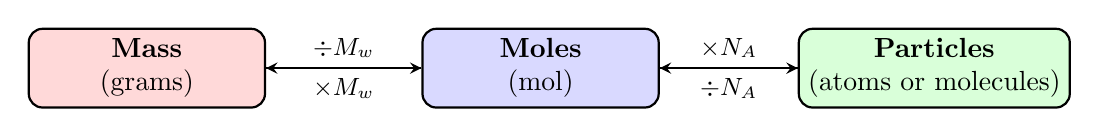
\begin{tikzpicture}[
        box/.style={rectangle, draw, thick, fill=#1, rounded corners=5pt, minimum width=3cm, minimum height=1cm, align=center},
        arr/.style={->, thick, >=stealth}
    ]
        \node[box=red!15] (masa) at (-5,0) {\textbf{Mass} \\ (grams)};
        \node[box=blue!15] (mol) at (0,0) {\textbf{Moles} \\ (mol)};
        \node[box=green!15] (part) at (5,0) {\textbf{Particles} \\ (atoms or molecules)};

        \draw[arr] (masa) -- node[above, font=\small] {\( \div M_w \)} (mol);
        \draw[arr] (mol) -- node[below, font=\small] {\( \times M_w \)} (masa);
        \draw[arr] (mol) -- node[above, font=\small] {\( \times N_A \)} (part);
        \draw[arr] (part) -- node[below, font=\small] {\( \div N_A \)} (mol);
    \end{tikzpicture}
    \caption{Relationship between mass, moles, and number of particles.}
    \label{fig:masa_mol_particulas}
\end{figure}

\begin{example}{}

    Calculate the moles of \ch{CH4} contained in \qty{48}{\g}.

    \datos{}: The atomic masses are: \( \ch{H} = 1 \); \( \ch{C} = 12 \).

    First we must calculate the molar mass. As we have said, the molar mass has the same numerical value as the molecular mass, but in \unit{\g\per\mole} instead of amu.

    \[
        \ch{CH4} \left\{\rule{0pt}{0.8cm}
                     \begin{array}{lcl}
                         \ch{H} &=& 4 \times \qty{1}{\uma} = \qty{4}{\uma} \\
                         \ch{C} &=& 1 \times \qty{12}{\uma} = \qty{12}{\uma} \\
                         \cline{1-3}
                         \multicolumn{3}{r}{\textbf{Total} = \qty{16}{\uma} }
                     \end{array}
        \right.
    \]

    Therefore, the molar mass of \ch{CH4} is \qty{16}{\g\per\mole}.

    Applying the formula:
    \begin{equation*}
        n = \dfrac{m}{M_w} = \dfrac{48}{16} = \qty{3}{\mole} \text{ of \ch{CH4}}
    \end{equation*}
\end{example}



\begin{exercise}
    A flask contains \qty{100}{\g} of calcium carbonate, \ch{CaCO3}. Calculate the amount of this substance, in moles, in that container.
    \begin{solu}
        A flask contains \qty{100}{\g} of calcium carbonate, \ch{CaCO3}. Calculate the amount of this substance, in moles, in that container.

        Calculate the moles in \qty{100}{\g} of \ch{CaCO3}.

        Atomic masses: \( \ch{Ca} = 40 \); \( \ch{C} = 12 \); \( \ch{O} = 16 \).

        Molar mass of \ch{CaCO3}: \( 40 + 12 + 3 \times 16 = \qty{100}{\g\per\mole} \).

        \begin{equation*}
            n = \dfrac{m}{M_w} = \dfrac{100}{100} = \qty{1}{\mole} \text{ of \ch{CaCO3}}
        \end{equation*}
    \end{solu}
\end{exercise}

\begin{exercise}
    What amount in moles of gaseous nitrogen, \ch{N2}, is in \qty{56}{\g} of this substance? How many molecules are there? And how many atoms?
    \begin{solu}
        What amount in moles of gaseous nitrogen, \ch{N2}, is in \qty{56}{\g} of this substance? How many molecules are there? And how many atoms?

        Calculate the moles, molecules, and atoms in \qty{56}{\g} of \ch{N2}.

        Atomic mass: \( \ch{N} = 14 \). Molar mass of \ch{N2}: \( 2 \times 14 = \qty{28}{\g\per\mole} \).

        \textbf{Moles:}
        \begin{equation*}
            n = \dfrac{56}{28} = \qty{2}{\mole} \text{ of \ch{N2}}
        \end{equation*}

        \textbf{Molecules:}
        \begin{equation*}
            2\ \cancelred{\unit{\mole}} \times \num{6.022e23}\ \dfrac{\text{molecules}}{\cancelred{\unit{\mole}}} = \num{12.044e23} = \num{1.2044e24} \text{ molecules of \ch{N2}}
        \end{equation*}

        \textbf{Atoms:} Each \ch{N2} molecule has 2 N atoms:
        \begin{equation*}
            \num{1.2044e24} \times 2 = \num{2.4088e24} \text{ atoms of N}
        \end{equation*}
    \end{solu}
\end{exercise}

\begin{exercise}
    Calculate the molar masses of the following substances: bromine (\ch{Br2}), potassium iodide (\ch{KI}), calcium carbonate (\ch{CaCO3}), and sodium carbonate (\ch{Na2CO3}).
    \begin{solu}
        Calculate the molar masses of the following substances: bromine (\ch{Br2}), potassium iodide (\ch{KI}), calcium carbonate (\ch{CaCO3}), and sodium carbonate (\ch{Na2CO3}).

        Calculate the molar masses of \ch{Br2}, \ch{KI}, \ch{CaCO3}, and \ch{Na2CO3}.

        Atomic masses: \( \ch{Br} = 80 \); \( \ch{K} = 39 \); \( \ch{I} = 127 \); \( \ch{Ca} = 40 \); \( \ch{C} = 12 \); \( \ch{O} = 16 \); \( \ch{Na} = 23 \).
        \begin{itemize}
            \item \ch{Br2}: \( 2 \times 80 = \qty{160}{\g\per\mole} \)
            \item \ch{KI}: \( 39 + 127 = \qty{166}{\g\per\mole} \)
            \item \ch{CaCO3}: \( 40 + 12 + 3 \times 16 = \qty{100}{\g\per\mole} \)
            \item \ch{Na2CO3}: \( 2 \times 23 + 12 + 3 \times 16 = 46 + 12 + 48 = \qty{106}{\g\per\mole} \)
        \end{itemize}
    \end{solu}
\end{exercise}

\begin{exercise}
    What amount of substance, in moles, is in \qty{66}{\g} of carbon dioxide, \ch{CO2}?
    \begin{solu}
        What amount of substance, in moles, is in \qty{66}{\g} of carbon dioxide, \ch{CO2}?

        Calculate the moles in \qty{66}{\g} of \ch{CO2}.

        Atomic masses: \( \ch{C} = 12 \); \( \ch{O} = 16 \).

        Molar mass of \ch{CO2}: \( 12 + 2 \times 16 = \qty{44}{\g\per\mole} \).

        \begin{equation*}
            n = \dfrac{66}{44} = \qty{1.5}{\mole} \text{ of \ch{CO2}}
        \end{equation*}
    \end{solu}
\end{exercise}

\begin{exercise}
    Calculate the mass of:
    \begin{enumerate}[label=\letraminuscula]
\item \qty{2}{\mole} of hydrogen chloride, \ch{HCl}.
\item \qty{2}{\mole} of water, \ch{H2O}.
\item \qty{1.5}{\mole} of sulfuric acid, \ch{H2SO4}.
\item \qty{0.5}{\mole} of chlorine, \ch{Cl2}.
    \end{enumerate}
    \begin{solu}
        Calculate the mass of:
        \begin{enumerate}[label=\letraminuscula]
\item \qty{2}{\mole} of hydrogen chloride, \ch{HCl}.
\item \qty{2}{\mole} of water, \ch{H2O}.
\item \qty{1.5}{\mole} of sulfuric acid, \ch{H2SO4}.
\item \qty{0.5}{\mole} of chlorine, \ch{Cl2}.
        \end{enumerate}

        Calculate the mass of each substance. We use \( m = n \times M_w \).

        Atomic masses: \( \ch{H} = 1 \); \( \ch{Cl} = 35{,}5 \); \( \ch{O} = 16 \); \( \ch{S} = 32 \).

        \begin{enumerate}[label=\letraminuscula]
\item \ch{HCl}: \( M_w = 1 + 35{,}5 = \qty{36.5}{\g\per\mole} \). \( m = 2 \times 36{,}5 = \qty{73}{\g} \).
\item \ch{H2O}: \( M_w = 2 \times 1 + 16 = \qty{18}{\g\per\mole} \). \( m = 2 \times 18 = \qty{36}{\g} \).
\item \ch{H2SO4}: \( M_w = 2 + 32 + 64 = \qty{98}{\g\per\mole} \). \( m = 1{,}5 \times 98 = \qty{147}{\g} \).
\item \ch{Cl2}: \( M_w = 2 \times 35{,}5 = \qty{71}{\g\per\mole} \). \( m = 0{,}5 \times 71 = \qty{35.5}{\g} \).
        \end{enumerate}
    \end{solu}
\end{exercise}

\begin{exercise}
    What amount in moles of substance is in \qty{36.5}{\g} of \ch{HCl}, in \qty{73}{\g} of \ch{HCl}, and in \qty{146}{\g} of \ch{HCl}?
    \begin{solu}
        What amount in moles of substance is in \qty{36.5}{\g} of \ch{HCl}, in \qty{73}{\g} of \ch{HCl}, and in \qty{146}{\g} of \ch{HCl}?

        Calculate the moles in \qty{36.5}{\g}, \qty{73}{\g}, and \qty{146}{\g} of \ch{HCl}.

        Molar mass of \ch{HCl}: \( 1 + 35{,}5 = \qty{36.5}{\g\per\mole} \).

        \begin{itemize}
            \item \( n = \dfrac{36{,}5}{36{,}5} = \qty{1}{\mole} \)
            \item \( n = \dfrac{73}{36{,}5} = \qty{2}{\mole} \)
            \item \( n = \dfrac{146}{36{,}5} = \qty{4}{\mole} \)
        \end{itemize}
    \end{solu}
\end{exercise}


\section{Ideal Gas Law}

The three gas laws (Gay-Lussac's Law, Charles's Law, and Boyle-Mariotte's Law) can be combined into a single law called the \textbf{Ideal Gas Law}. This law relates pressure, volume, and temperature with the amount of substance in moles.

The mathematical expression of this law is:
\vspace{20pt}
\begin{centeredequation}
    \eqnmarkbox[blue]{presion}{p}
    \cdot
    \eqnmarkbox[red]{volumen}{V}
    =
    \eqnmarkbox[mDarkTeal]{moles}{n}
    \cdot
    \eqnmarkbox[orange]{constante}{R}
    \cdot
    \eqnmarkbox[violet]{temperatura}{T}
\end{centeredequation}
\vspace{25pt}
\annotate[yshift=1em]{left}{presion}{Pressure in \unit{\atmosphere}}
\annotate[yshift=-0.5em]{below,left}{volumen}{Volume in \unit{\litre}}
\annotate[yshift=1em]{}{moles}{number of moles}
\annotate[yshift=-2em]{below,left}{constante}{Ideal gas constant; R = \ctegases{}}
\annotate[yshift=-1em]{below}{temperatura}{Temperature in \unit{\kelvin}}
\begin{exercise}
    We have \qty{3}{\mole} of an ideal gas at a temperature of \qty{300}{\kelvin} and a pressure of \qty{2}{\atmosphere}. Calculate the volume occupied by the gas.
    \begin{solu}
        We have \qty{3}{\mole} of an ideal gas at a temperature of \qty{300}{\kelvin} and a pressure of \qty{2}{\atmosphere}. Calculate the volume occupied by the gas.

        Calculate the volume of \qty{3}{\mole} of gas at \qty{300}{\kelvin} and \qty{2}{\atmosphere}.

        We solve for \( V \) from the ideal gas law:
        \begin{equation*}
            V = \dfrac{nRT}{p} = \dfrac{3 \times 0{,}082 \times 300}{2} = \dfrac{73{,}8}{2} = \qty{36.9}{\litre}
        \end{equation*}
    \end{solu}
\end{exercise}
\begin{exercise}
    An ideal gas occupies a volume of \qty{10}{\litre} at a pressure of \qty{1.5}{\atmosphere} and a temperature of \qty{350}{\kelvin}. How many moles of gas are there?
    \begin{solu}
        An ideal gas occupies a volume of \qty{10}{\litre} at a pressure of \qty{1.5}{\atmosphere} and a temperature of \qty{350}{\kelvin}. How many moles of gas are there?

        Calculate the moles of a gas that occupies \qty{10}{\litre} at \qty{1.5}{\atmosphere} and \qty{350}{\kelvin}.

        We solve for \( n \):
        \begin{equation*}
            n = \dfrac{pV}{RT} = \dfrac{1{,}5 \times 10}{0{,}082 \times 350} = \dfrac{15}{28{,}7} = \qty{0.52}{\mole}
        \end{equation*}
    \end{solu}
\end{exercise}
\begin{exercise}
    What is the volume in mL occupied by an ideal gas if \qty{0.553}{\mol} are at a temperature of \qty{1226.49}{\kelvin} and a pressure of \qty{4935}{\mmHg}?
    \begin{solu}
        What is the volume in mL occupied by an ideal gas if \qty{0.553}{\mol} are at a temperature of \qty{1226.49}{\kelvin} and a pressure of \qty{4935}{\mmHg}?

        We apply the ideal gas law $PV = nRT$, solving for volume:
        \begin{equation*}
            V = \frac{nRT}{P}
        \end{equation*}
        \textbf{Step 1: Identify the data.}
        \begin{align*}
            n &= \qty{0.553}{\mol} \\
            T &= \qty{1226.49}{\kelvin} \\
            P &= \qty{4935}{\mmHg} \\
            R &= \qty{0.082057}{\atm\liter\per\mol\per\kelvin}
        \end{align*}
        \textbf{Step 2: Convert the pressure to atm.}

        The constant $R$ is expressed in atm units, so we must convert the pressure from mmHg to atm using the conversion factor $\qty{1}{\atm} = \qty{760}{\mmHg}$:
        \begin{equation*}
            P = \qty{4935}{\mmHg} \times \frac{\qty{1}{\atm}}{\qty{760}{\mmHg}} = \qty{6.4934}{\atm}
        \end{equation*}
        \textbf{Step 3: Substitute into the equation and calculate $V$ in liters.}
        \begin{equation*}
            V = \frac{nRT}{P} = \frac{\qty{0.553}{\mol} \times \qty{0.082057}{\atm\liter\per\mol\per\kelvin} \times \qty{1226.49}{\kelvin}}{\qty{6.4934}{\atm}} = \qty{8.573}{\liter}
        \end{equation*}
        \textbf{Step 4: Convert the volume to mL.}

        Since the problem asks for the volume in mL, we use the conversion factor $\qty{1}{\liter} = \qty{1000}{\mL}$:
        \begin{equation*}
            V = \qty{8.573}{\liter} \times \frac{\qty{1000}{\mL}}{\qty{1}{\liter}} = \boxed{\qty{8573}{\mL}}
        \end{equation*}
    \end{solu}
\end{exercise}
\begin{exercise}
    What is the temperature in \unit{\kelvin} of an ideal gas, if \qty{0.405}{\mole} occupy a volume of \qty{7720}{\mL} at a pressure of \qty{790}{\mmHg}?
    \begin{solu}
        What is the temperature in \unit{\kelvin} of an ideal gas, if \qty{0.405}{\mole} occupy a volume of \qty{7720}{\mL} at a pressure of \qty{790}{\mmHg}?

        We apply the ideal gas law $PV = nRT$, solving for temperature:
        \begin{equation*}
            T = \frac{PV}{nR}
        \end{equation*}
        \textbf{Step 1: Identify the data.}
        \begin{align*}
            n &= \qty{0.405}{\mol} \\
            V &= \qty{7720}{\mL} \\
            P &= \qty{790}{\mmHg} \\
            R &= \qty{0.082057}{\atm\liter\per\mol\per\kelvin}
        \end{align*}
        \textbf{Step 2: Convert the pressure to atm.}

        We convert mmHg to atm using the conversion factor $\qty{1}{\atm} = \qty{760}{\mmHg}$:
        \begin{equation*}
            P = \qty{790}{\mmHg} \times \frac{\qty{1}{\atm}}{\qty{760}{\mmHg}} = \qty{1.03947}{\atm}
        \end{equation*}
        \textbf{Step 3: Convert the volume to liters.}

        The constant $R$ has liters in its units, so we convert mL to L using the conversion factor $\qty{1}{\liter} = \qty{1000}{\mL}$:
        \begin{equation*}
            V = \qty{7720}{\mL} \times \frac{\qty{1}{\liter}}{\qty{1000}{\mL}} = \qty{7.720}{\liter}
        \end{equation*}
        \textbf{Step 4: Substitute into the equation and calculate $T$.}
        \begin{equation*}
            T = \frac{PV}{nR} = \frac{\qty{1.03947}{\atm} \times \qty{7.720}{\liter}}{\qty{0.405}{\mol} \times \qty{0.082057}{\atm\liter\per\mol\per\kelvin}} = \boxed{\qty{241.5}{\kelvin}}
        \end{equation*}
    \end{solu}
\end{exercise}
\begin{exercise}
    What is the temperature in \unit{\degreeCelsius} of an ideal gas, if \qty{0.746}{\mol} occupy a volume of \qty{9890}{\mL} at a pressure of \qty{1.41}{\atmosphere}?
    \begin{solu}
        What is the temperature in \unit{\degreeCelsius} of an ideal gas, if \qty{0.746}{\mol} occupy a volume of \qty{9890}{\mL} at a pressure of \qty{1.41}{\atmosphere}?

        We apply the ideal gas law $PV = nRT$, solving for temperature:
        \begin{equation*}
            T = \frac{PV}{nR}
        \end{equation*}
        \textbf{Step 1: Identify the data.}
        \begin{align*}
            n &= \qty{0.746}{\mol} \\
            V &= \qty{9890}{\mL} \\
            P &= \qty{1.41}{\atm} \\
            R &= \qty{0.082057}{\atm\liter\per\mol\per\kelvin}
        \end{align*}
        \textbf{Step 2: Convert the volume to liters.}

        We convert mL to L using the conversion factor $\qty{1}{\liter} = \qty{1000}{\mL}$:
        \begin{equation*}
            V = \qty{9890}{\mL} \times \frac{\qty{1}{\liter}}{\qty{1000}{\mL}} = \qty{9.890}{\liter}
        \end{equation*}
        \textbf{Step 3: Substitute into the equation and calculate $T$ in Kelvin.}
        \begin{equation*}
            T = \frac{PV}{nR} = \frac{\qty{1.41}{\atm} \times \qty{9.890}{\liter}}{\qty{0.746}{\mol} \times \qty{0.082057}{\atm\liter\per\mol\per\kelvin}} = \qty{227.8}{\kelvin}
        \end{equation*}
        \textbf{Step 4: Convert the temperature to \unit{\degreeCelsius}.}

        The problem asks for the temperature in \unit{\degreeCelsius}. We use the relationship $T(\unit{\degreeCelsius}) = T(\unit{\kelvin}) - 273.15$:
        \begin{equation*}
            T = \qty{227.8}{\kelvin} - \qty{273.15}{\kelvin} = \boxed{\qty{-45.35}{\degreeCelsius}}
        \end{equation*}
    \end{solu}
\end{exercise}
\begin{exercise}
    What is the pressure in atm of an ideal gas if \qty{0.532}{\mol} occupy a volume of \qty{4390}{\mL} at a temperature of \qty{183.93}{\kelvin}?
    \begin{solu}
        What is the pressure in atm of an ideal gas if \qty{0.532}{\mol} occupy a volume of \qty{4390}{\mL} at a temperature of \qty{183.93}{\kelvin}?

        We apply the ideal gas law $PV = nRT$, solving for pressure:
        \begin{equation*}
            P = \frac{nRT}{V}
        \end{equation*}
        \textbf{Step 1: Identify the data.}
        \begin{align*}
            n &= \qty{0.532}{\mol} \\
            V &= \qty{4390}{\mL} \\
            T &= \qty{183.93}{\kelvin} \\
            R &= \qty{0.082057}{\atm\liter\per\mol\per\kelvin}
        \end{align*}
        \textbf{Step 2: Convert the volume to liters.}

        We convert mL to L using the conversion factor $\qty{1}{\liter} = \qty{1000}{\mL}$:
        \begin{equation*}
            V = \qty{4390}{\mL} \times \frac{\qty{1}{\liter}}{\qty{1000}{\mL}} = \qty{4.390}{\liter}
        \end{equation*}
        \textbf{Step 3: Substitute into the equation and calculate $P$.}
        \begin{equation*}
            P = \frac{nRT}{V} = \frac{\qty{0.532}{\mol} \times \qty{0.082057}{\atm\liter\per\mol\per\kelvin} \times \qty{183.93}{\kelvin}}{\qty{4.390}{\liter}} = \boxed{\qty{1.829}{\atm}}
        \end{equation*}
    \end{solu}
\end{exercise}
\begin{exercise}
    How many moles of an ideal gas are in a volume of \qty{4220}{\mL} if the temperature is \qty{279.35}{\kelvin} and the pressure is \qty{1.75}{\atmosphere}?
    \begin{solu}
        How many moles of an ideal gas are in a volume of \qty{4220}{\mL} if the temperature is \qty{279.35}{\kelvin} and the pressure is \qty{1.75}{\atmosphere}?

        We apply the ideal gas law $PV = nRT$, solving for the number of moles:
        \begin{equation*}
            n = \frac{PV}{RT}
        \end{equation*}
        \textbf{Step 1: Identify the data.}
        \begin{align*}
            V &= \qty{4220}{\mL} \\
            T &= \qty{279.35}{\kelvin} \\
            P &= \qty{1.75}{\atm} \\
            R &= \qty{0.082057}{\atm\liter\per\mol\per\kelvin}
        \end{align*}
        \textbf{Step 2: Convert the volume to liters.}

        We convert mL to L using the conversion factor $\qty{1}{\liter} = \qty{1000}{\mL}$:
        \begin{equation*}
            V = \qty{4220}{\mL} \times \frac{\qty{1}{\liter}}{\qty{1000}{\mL}} = \qty{4.220}{\liter}
        \end{equation*}
        \textbf{Step 3: Substitute into the equation and calculate $n$.}
        \begin{equation*}
            n = \frac{PV}{RT} = \frac{\qty{1.75}{\atm} \times \qty{4.220}{\liter}}{\qty{0.082057}{\atm\liter\per\mol\per\kelvin} \times \qty{279.35}{\kelvin}} = \boxed{\qty{0.3223}{\mol}}
        \end{equation*}
    \end{solu}
\end{exercise}

\subsection{Standard conditions (STP)}

In chemistry, it is very common to talk about standard conditions.
When we talk about standard conditions, we refer to pressure of \qty{1}{\atmosphere} and a temperature of \qty{0}{\degreeCelsius} (\qty{273}{\kelvin}).

It is important to know that \qty{1}{\mol} of \textbf{any gas} under standard conditions always occupies a volume of \qty{22.4}{\litre}. This volume is called the \textbf{molar volume}.

To verify this value, we just need to apply the ideal gas equation with \( n=1 \), \( p = \qty{1}{\atmosphere} \), and \( T = \qty{273}{\kelvin} \):
\begin{centeredequation}
    V = \dfrac{nRT}{p} = \dfrac{1 \times 0{,}082 \times 273}{1} = \qty{22.4}{\litre}
\end{centeredequation}
\begin{exercise}
    What volume do \qty{2}{\mole} of oxygen (\ch{O2}) occupy under standard conditions?
    \begin{solu}
        What volume do \qty{2}{\mole} of oxygen (\ch{O2}) occupy under standard conditions?

        Volume of \qty{2}{\mole} of \ch{O2} at STP.

        Under standard conditions, 1 mole of any gas occupies \qty{22.4}{\litre}:
        \begin{equation*}
            V = 2\ \cancelred{\unit{\mole}} \times \dfrac{\qty{22.4}{\litre}}{1\ \cancelred{\unit{\mole}}} = \qty{44.8}{\litre}
        \end{equation*}
    \end{solu}
\end{exercise}
\begin{exercise}
    How many moles of an ideal gas are in \qty{11.2}{\litre} under standard conditions?
    \begin{solu}
        How many moles of an ideal gas are in \qty{11.2}{\litre} under standard conditions?

        Moles in \qty{11.2}{\litre} of gas at STP.

        \begin{equation*}
            n = \dfrac{11{,}2}{22{,}4} = \qty{0.5}{\mole}
        \end{equation*}
    \end{solu}
\end{exercise}
\begin{exercise}
    What is the volume in mL occupied by \qty{0.553}{\mol} of an ideal gas at STP?
    \begin{solu}
        What is the volume in mL occupied by \qty{0.553}{\mol} of an ideal gas at STP?

        Standard conditions (STP) correspond to a temperature of $T = \qty{273.15}{\kelvin}$
        and a pressure of $P = \qty{1}{\atm}$. Under these conditions, we can calculate the
        molar volume of an ideal gas from the ideal gas law $PV = nRT$:
        \begin{equation*}
            V_m = \frac{RT}{P} = \frac{\qty{0.082057}{\atm\liter\per\mol\per\kelvin}
            \times \qty{273.15}{\kelvin}}{\qty{1}{\atm}} = \qty{22.414}{\liter\per\mol}
        \end{equation*}
        This value is known as the \textbf{molar volume at standard conditions} and allows
        us to directly calculate the volume of any amount of ideal gas at STP using the
        relationship:
        \begin{equation*}
            V = n \times V_m
        \end{equation*}
        \textbf{Step 1: Identify the data.}
        \begin{align*}
            n   &= \qty{0.553}{\mol} \\
            V_m &= \qty{22.414}{\liter\per\mol}
        \end{align*}
        \textbf{Step 2: Calculate the volume in liters.}
        \begin{equation*}
            V = n \times V_m = \qty{0.553}{\mol} \times \qty{22.414}{\liter\per\mol}
            = \qty{12.395}{\liter}
        \end{equation*}
        \textbf{Step 3: Convert the volume to mL.}

        The problem asks for the volume in mL, so we use the conversion factor
        $\qty{1}{\liter} = \qty{1000}{\mL}$:
        \begin{equation*}
            V = \qty{12.395}{\liter} \times \frac{\qty{1000}{\mL}}{\qty{1}{\liter}}
            = \boxed{\qty{12395}{\mL}}
        \end{equation*}
    \end{solu}
\end{exercise}
\begin{exercise}
    How many moles of an ideal gas are in a volume of \qty{7720}{\mL} at STP?
    \begin{solu}
        How many moles of an ideal gas are in a volume of \qty{7720}{\mL} at STP?

        Under standard conditions (STP), $T = \qty{273.15}{\kelvin}$ and $P = \qty{1}{\atm}$,
        the molar volume of an ideal gas is $V_m = \qty{22.414}{\liter\per\mol}$. Solving
        for the number of moles from the relationship $V = n \times V_m$:
        \begin{equation*}
            n = \frac{V}{V_m}
        \end{equation*}
        \textbf{Step 1: Identify the data.}
        \begin{align*}
            V   &= \qty{7720}{\mL} \\
            V_m &= \qty{22.414}{\liter\per\mol}
        \end{align*}
        \textbf{Step 2: Convert the volume to liters.}

        The constant $V_m$ is expressed in \unit{\liter\per\mol}, so we must convert
        the volume from mL to L using the conversion factor
        $\qty{1}{\liter} = \qty{1000}{\mL}$:
        \begin{equation*}
            V = \qty{7720}{\mL} \times \frac{\qty{1}{\liter}}{\qty{1000}{\mL}}
            = \qty{7.720}{\liter}
        \end{equation*}
        \textbf{Step 3: Calculate the number of moles.}
        \begin{equation*}
            n = \frac{V}{V_m} = \frac{\qty{7.720}{\liter}}{\qty{22.414}{\liter\per\mol}}
            = \boxed{\qty{0.3444}{\mol}}
        \end{equation*}
    \end{solu}
\end{exercise}
\begin{exercise}
    What is the volume in \unit{\liter} occupied by \qty{0.746}{\mol} of an ideal gas at STP?
    \begin{solu}
        What is the volume in \unit{\liter} occupied by \qty{0.746}{\mol} of an ideal gas at STP.

        \negsubro{SOLUTION:}

        Under standard conditions (STP), $T = \qty{273.15}{\kelvin}$ and $P = \qty{1}{\atm}$,
        the molar volume of an ideal gas is $V_m = \qty{22.414}{\liter\per\mol}$. The volume
        occupied by an amount $n$ of ideal gas is calculated using:
        \begin{equation*}
            V = n \times V_m
        \end{equation*}
        \textbf{Step 1: Identify the data.}
        \begin{align*}
            n   &= \qty{0.746}{\mol} \\
            V_m &= \qty{22.414}{\liter\per\mol}
        \end{align*}
        \textbf{Step 2: Calculate the volume in liters.}

        Since the problem asks for the result directly in liters, no unit conversion is
        necessary:
        \begin{equation*}
            V = n \times V_m = \qty{0.746}{\mol} \times \qty{22.414}{\liter\per\mol}
            = \boxed{\qty{16.721}{\liter}}
        \end{equation*}
    \end{solu}
\end{exercise}
\begin{exercise}
    How many moles of an ideal gas are in a volume of \qty{4390}{\mL} at STP?
    \begin{solu}
        How many moles of an ideal gas are in a volume of \qty{4390}{\mL} at STP?

        \negsubro{SOLUTION:}

        Under standard conditions (STP), $T = \qty{273.15}{\kelvin}$ and $P = \qty{1}{\atm}$,
        the molar volume of an ideal gas is $V_m = \qty{22.414}{\liter\per\mol}$. Solving
        for the number of moles from the relationship $V = n \times V_m$:
        \begin{equation*}
            n = \frac{V}{V_m}
        \end{equation*}
        \textbf{Step 1: Identify the data.}
        \begin{align*}
            V   &= \qty{4390}{\mL} \\
            V_m &= \qty{22.414}{\liter\per\mol}
        \end{align*}
        \textbf{Step 2: Convert the volume to liters.}

        We convert mL to L using the conversion factor $\qty{1}{\liter} = \qty{1000}{\mL}$:
        \begin{equation*}
            V = \qty{4390}{\mL} \times \frac{\qty{1}{\liter}}{\qty{1000}{\mL}}
            = \qty{4.390}{\liter}
        \end{equation*}
        \textbf{Step 3: Calculate the number of moles.}
        \begin{equation*}
            n = \frac{V}{V_m} = \frac{\qty{4.390}{\liter}}{\qty{22.414}{\liter\per\mol}}
            = \boxed{\qty{0.1959}{\mol}}
        \end{equation*}
    \end{solu}
\end{exercise}
\begin{exercise}
    What is the volume in mL occupied by \qty{1.75}{\mol} of an ideal gas at STP?
    \begin{solu}
        What is the volume in mL occupied by \qty{1.75}{\mol} of an ideal gas at STP?

        \negsubro{SOLUTION:}

        Under standard conditions (STP), $T = \qty{273.15}{\kelvin}$ and $P = \qty{1}{\atm}$,
        the molar volume of an ideal gas is $V_m = \qty{22.414}{\liter\per\mol}$. The volume
        occupied by an amount $n$ of ideal gas is calculated using:
        \begin{equation*}
            V = n \times V_m
        \end{equation*}
        \textbf{Step 1: Identify the data.}
        \begin{align*}
            n   &= \qty{1.75}{\mol} \\
            V_m &= \qty{22.414}{\liter\per\mol}
        \end{align*}
        \textbf{Step 2: Calculate the volume in liters.}
        \begin{equation*}
            V = n \times V_m = \qty{1.75}{\mol} \times \qty{22.414}{\liter\per\mol}
            = \qty{39.225}{\liter}
        \end{equation*}
        \textbf{Step 3: Convert the volume to mL.}

        The problem asks for the volume in mL, so we use the conversion factor
        $\qty{1}{\liter} = \qty{1000}{\mL}$:
        \begin{equation*}
            V = \qty{39.225}{\liter} \times \frac{\qty{1000}{\mL}}{\qty{1}{\liter}}
            = \boxed{\qty{39225}{\mL}}
        \end{equation*}
    \end{solu}
\end{exercise}


\section{Vocabulary}

\begin{vocabulary}[Valence electrons]
    Electrons in the outermost shell of an atom which are responsible for the chemical properties of an element. \newline
    \textbf{Translation to Spanish}: Electrones de valencia \newline
    % 248
\end{vocabulary}

\begin{vocabulary}[Chemical compound]
    Substance formed by two or more different elements that are chemically bonded together in fixed and specific proportions. \newline
    \textbf{Translation to Spanish}: Compuesto químico \newline
    % 271
\end{vocabulary}

\begin{vocabulary}[Molecule]
    The smallest possible unit of a chemical substance that still retains all of its unique and characteristic properties. \newline
    \textbf{Translation to Spanish}: Molécula \newline
    % 273
\end{vocabulary}

\begin{vocabulary}[Isolated atoms]
    Atoms found in noble gases that do not tend to combine with others because their valence shell is complete. \newline
    \textbf{Translation to Spanish}: Átomos aislados \newline
    % 275
\end{vocabulary}

\begin{vocabulary}[Noble gases]
    Highly stable elements that do not conduct electricity or react with other substances due to their complete shells. \newline
    \textbf{Translation to Spanish}: Gases nobles \newline
    % 276
\end{vocabulary}

\begin{vocabulary}[Homonuclear diatomic molecules]
    Molecules formed by the union of two atoms of the same chemical element, such as oxygen or hydrogen. \newline
    \textbf{Translation to Spanish}: Moléculas diatómicas homonucleares \newline
    % 280
\end{vocabulary}

\begin{vocabulary}[Heteronuclear molecules]
    Specific types of molecules that contain two or more different elements chemically bonded together in a single unit. \newline
    \textbf{Translation to Spanish}: Moléculas heteronucleares \newline
    % 282
\end{vocabulary}

\begin{vocabulary}[Crystals]
    Solids whose internal particles are arranged following a pattern that repeats in all three dimensions of physical space. \newline
    \textbf{Translation to Spanish}: Cristales \newline
    % 283
\end{vocabulary}

\begin{vocabulary}[Chemical bond]
    The union between atoms of different elements that occurs because the molecule formed is more stable than others. \newline
    \textbf{Translation to Spanish}: Enlace químico \newline
    % 317
\end{vocabulary}

\begin{vocabulary}[Ionic bond]
    Bond that occurs by electron transfer where one element loses electrons and another gains them, forming stable ions. \newline
    \textbf{Translation to Spanish}: Enlace iónico \newline
    % 318
\end{vocabulary}

\begin{vocabulary}[Cation]
    A positive ion formed when a neutral atom loses one or more electrons during a chemical reaction process. \newline
    \textbf{Translation to Spanish}: Catión \newline
    % 319
\end{vocabulary}

\begin{vocabulary}[Anion]
    A negative ion formed when a neutral atom gains one or more electrons during a chemical reaction process. \newline
    \textbf{Translation to Spanish}: Anión \newline
    % 319
\end{vocabulary}

\begin{vocabulary}[Covalent bond]
    The specific type of chemical bond that forms when two atoms share electrons to complete their outermost shell. \newline
    \textbf{Translation to Spanish}: Enlace covalente \newline
    % 343
\end{vocabulary}

\begin{vocabulary}[Metallic bond]
    Bond between atoms of metallic elements where valence electrons move freely, forming a large and common electron cloud. \newline
    \textbf{Translation to Spanish}: Enlace metálico \newline
    % 364
\end{vocabulary}

\begin{vocabulary}[Electron cloud]
    The zone in metallic bonds where valence electrons move freely among all the atoms, allowing electrical conduction. \newline
    \textbf{Translation to Spanish}: Nube electrónica \newline
    % 364
\end{vocabulary}

\begin{vocabulary}[Graphite]
    A non-metallic crystal formed by carbon atoms arranged in stacked hexagonal layers that are soft and opaque. \newline
    \textbf{Translation to Spanish}: Grafito \newline
    % 296
\end{vocabulary}
    

